\documentclass[11pt,a4paper]{ctexart}
\usepackage[margin=2.2cm]{geometry}
\usepackage{graphicx}
\usepackage{booktabs}
\usepackage{longtable}
\usepackage{array}
\usepackage{enumitem}
\usepackage{xcolor}
\usepackage{tikz}
\usetikzlibrary{arrows.meta,positioning,shapes.geometric,shapes.multipart,fit,backgrounds,calc}
\usepackage{listings}
\usepackage{caption}
\usepackage{adjustbox}
\usepackage[section]{placeins}
\usepackage{needspace}
\usepackage{hyperref}
\hypersetup{colorlinks=true,linkcolor=blue!50!black,urlcolor=blue!50!black}
\setlist{itemsep=2pt,topsep=3pt}
\captionsetup{font=small}

\sloppy
\setlength{\emergencystretch}{4em}

\lstset{
  basicstyle=\ttfamily\footnotesize,
  keywordstyle=\color{blue!60!black},
  commentstyle=\color{green!40!black},
  frame=single,
  rulecolor=\color{gray!50},
  breaklines=true,
  showstringspaces=false,
  xleftmargin=4pt,
  xrightmargin=4pt
}

\newcommand{\cl}[1]{\texttt{#1}}

% ---- boites de classe UML : trois compartiments, largeur et alignement maitrises ----
\definecolor{umlBord}{RGB}{139,32,74}
\definecolor{umlFill}{RGB}{252,246,214}
\tikzset{
  umlclass/.style={%
    draw=umlBord, fill=umlFill, text=black, line width=0.6pt,
    rectangle split, rectangle split parts=3,
    rectangle split part align={center,left,left},
    align=left, font=\scriptsize, inner xsep=3.5pt, inner ysep=2.8pt},
  umlline/.style={draw=umlBord, line width=0.6pt},
  umlgen/.style={umlline, -{Triangle[open, length=7pt, width=6pt]}},
  umlagg/.style={umlline, {Diamond[open, length=8pt, width=6pt]}-},
  umlcomp/.style={umlline, {Diamond[length=8pt, width=6pt]}-},
  umlmult/.style={font=\scriptsize, fill=white, inner sep=1pt, text=black}
}
% \umlbox{identifiant}{titre}{position}{largeur}{attributs}{operations}
\newcommand{\umlbox}[6]{%
  \node[umlclass, text width=#4] (#1) at (#3)
    {\textbf{#2}\nodepart{second}#5\nodepart{third}#6};%
}

\title{\textbf{LO02 --- Projet Codex Naturalis}\\[4pt]
\large 基于课程所授 C++ 与设计模式的控制台实现\\[2pt]
\large Rapport de projet}
\author{24122608 袁鹏杰 \quad 24122603 刘羽骋 \quad 24123026 张浩冉\\[2pt]
24124237 梁皓 \quad 24123948 王蕊\\[6pt]
Université de Technologie Sino-Européenne de l'Université de Shanghai}
\date{2026 年 12 月}

\begin{document}
\maketitle
\thispagestyle{empty}

\vspace{6mm}
\begin{center}
\begin{tabular}{ll}
\toprule
课程 & LO02 --- Principes et pratique de la programmation orientée objet \\
学年 & 2026--2027 秋季学期（A26）\\
游戏 & Codex Naturalis（Thomas Dupont / Bombyx）\\
实现方式 & C++14，控制台界面，无第三方库 \\
代码规模 & 约 4\,900 行 C++（\cl{src/}，含头文件）+ 约 610 行测试 \\
视频链接 & \cl{【在此处填写 bilibili 链接】} \\
提交日期 & 2026-12-28 \\
\bottomrule
\end{tabular}
\end{center}

\vspace{8mm}
\begin{quote}
\textbf{摘要。}本项目用课程所讲授的 C++ 语言与面向对象设计方法，完整实现了桌游
\emph{Codex Naturalis} 的控制台版本。程序支持 1--4 名玩家（真人与电脑混合）、
严格的放置与资源校验、三类镀金牌的即时计分、四类目标卡的终局计分，以及完整的终局判定。
架构上使用课程出现过的语言特性与七个设计模式（Template Method、Strategy、
Factory Method、Singleton、Iterator、Adapter、Composite），并通过自动化脚本证明：全部源码在 \cl{-Wall -Wextra -pedantic} 下零警告，
\cl{c++14}/\cl{c++17} 均可编译，207 次断言全部通过，200 局自动对局无异常。
\end{quote}

\newpage
\tableofcontents
\newpage

\section{项目概述}

\subsection{游戏简介}
\emph{Codex Naturalis} 是一款二人以上（可单人）的卡牌摆放游戏。玩家扮演缮写修士，
要把「活页」拼接成自己的手稿：每张牌有四个角落，角落上可能印有四种王国资源
（植物、动物、真菌、昆虫）、三种物件（羽毛、墨水瓶、羊皮纸），也可能是「空角」或「缺失角」。
玩家每回合把手牌放一张到自己的区域，再抽一张新牌。放牌必须覆盖场上已有的一个
可见角落，而且不能同时覆盖同一张牌的两个角落——这就形成了「用资源换空间」的核心张力：
覆盖会盖掉自己已有的资源，但也让区域继续生长。

得分有两条线：一是放牌当下的即时分（资源牌可能带 1 分；镀金牌按固定分、
按覆盖的角落数、或按场上物件数计分）；二是终局的目标卡分
（2 张公共目标 + 1 张秘密目标，分别按斜线、L 型、三同资源、物件对/三异等图案计分）。
先到 20 分或两个牌堆抽空触发终局：补完本轮、每人最后一回合，然后结算目标分。

\subsection{项目目标与成功标准}
\begin{enumerate}
\item \textbf{功能完整}：开局参数化（人数与姓名）、动作合法性校验、终局判定、计分与胜负判定，
      控制台画面足以理解局面。
\item \textbf{架构可扩展}：新增 AI、新增目标类型、新增牌类或新增显示方式时，
      不修改既有的规则代码。
\item \textbf{严守课程范围}：只使用课程出现过的语言特性与设计模式，不用任何第三方库。
\item \textbf{可验证}：单元测试、批量自动对局、静态检查三条线全部可复现。
\end{enumerate}


\section{功能实现情况}

表 \ref{tab:fonctions} 逐条对照作业要求。所有要求的功能均已实现，并由
\cl{codex\_tests.exe} 中的用例覆盖。

\begin{table}[h]
\centering
\small
\begin{tabular}{p{5.4cm}p{1.5cm}p{7.6cm}}
\toprule
作业要求的功能 & 状态 & 实现位置与说明 \\
\midrule
开局参数化（人数、姓名） & 已完成 & \cl{Menu}：1--4 人、每座位姓名、真人/电脑、AI 难度 \\
单人/多人模式 & 已完成 & 1 人即「1 真人 + IA」；每座位可独立设为电脑 \\
初始牌选面 & 已完成 & \cl{Partie::choisirFaceInitiale}；界面同时显示正反两面的角与中央资源 \\
秘密目标二选一 & 已完成 & \cl{Partie::choisirObjectifSecret}（2 张候选） \\
放牌合法性校验 & 已完成 & \cl{ZoneDeJeu::placementValide}：可见角、隐藏角、重叠、镀金资源 \\
抽牌合法性校验 & 已完成 & \cl{Partie::piocher}：4 张明牌或两牌堆；非法来源抛异常 \\
终局判定 & 已完成 & 20 分或两牌堆空；补轮 + 最后一回合 \\
即时计分 & 已完成 & 资源牌横幅分、镀金牌固定分/按角/按物件 \\
目标计分 & 已完成 & 斜线、L、三同资源、物件对与三异 \\
胜负与平局 & 已完成 & 总分 $\rightarrow$ 目标分 $\rightarrow$ 并列 \\
控制台局面显示 & 已完成 & \cl{VueConsole}：角标网格 + 已放牌清单 + 资源/物件统计 + 手牌详情 \\
\bottomrule
\end{tabular}
\caption{功能需求与实现对照}
\label{tab:fonctions}
\end{table}

\section{总体架构}

\subsection{分层与依赖方向}
项目分为四层（图 \ref{fig:archi}）：
\cl{noyau}（与业务无关的工具：资源枚举、坐标、随机数、异常、洗牌模板）、
\cl{modele}（全部规则：\cl{Partie}、\cl{Joueur}、\cl{ZoneDeJeu}、\cl{Pioche}、
卡牌与目标层次、\cl{CatalogueCartes}、\cl{StrategieIA}）、
\cl{vue}（显示：抽象 \cl{Vue} 与控制台实现）、
\cl{controleur}（交互：菜单、主循环、输入适配、自动回合、批量模拟）。
依赖方向严格单向：\cl{main} $\rightarrow$ \cl{controleur} $\rightarrow$
\{\cl{modele}, \cl{vue}\} $\rightarrow$ \cl{noyau}。

最关键的设计决定是：\textbf{模型层不做任何输入输出}。\cl{Partie} 只接收
「放这张牌到这个位置」「从那里抽一张」这样的动作，要么成功、要么抛出
\cl{ExceptionJeu} 子类且状态不变。因此：
\begin{itemize}
\item 引擎可以被测试直接驱动（不需要模拟键盘）；
\item 换一套界面（图形界面、网络）不需要改规则；
\item 相同种子的对局完全可复现，便于回归测试。
\end{itemize}

\begin{figure}[h]
\centering
\begin{adjustbox}{max width=\linewidth}
\begin{tikzpicture}[node distance=6mm, font=\small,
  couche/.style={draw, rounded corners, fill=blue!6, align=center, text width=10.2cm, minimum height=9mm}]
\node[couche] (main) {\cl{main.cpp}：命令行参数、选择交互模式或自动模式};
\node[couche, below=of main] (ctrl) {\cl{controleur/}：Menu、ControleurPartie、Saisie 与 AdaptateurFlux、TourAutomatique、SimulationIA};
\node[couche, below=of ctrl] (vue) {\cl{vue/}：\cl{Vue}（抽象接口）$\Rightarrow$ \cl{VueConsole}（控制台实现）};
\node[couche, below=of vue] (model) {\cl{modele/}：Partie、Joueur、ZoneDeJeu、Pioche、Carte 层次、Objectif 层次、CatalogueCartes、StrategieIA};
\node[couche, below=of model, fill=gray!10] (noyau) {\cl{noyau/}：Ressource、Coin、Coordonnee、GenerateurAleatoire、ExceptionJeu、Melange};
\draw[-{Latex}] (main) -- (ctrl);
\draw[-{Latex}] (ctrl) -- (vue);
\draw[-{Latex}] (vue.south) -- (model.north);
\draw[-{Latex}] (model) -- (noyau);
\node[right=1mm of ctrl.east, align=left, font=\scriptsize, text=gray] {单向依赖};
\end{tikzpicture}
\end{adjustbox}
\caption{四层架构与单向依赖}
\label{fig:archi}
\end{figure}

\subsection{一次回合的交互时序}
图 \ref{fig:seq} 给出一名真人玩家放一张牌的完整交互：控制器先让视图打印局面，
再依次询问手牌编号、正反面与落点；模型在真正修改状态之前完成全部校验，
因此任何一次拒绝都不会破坏对局状态。

\begin{figure}[h]
\centering
\begin{adjustbox}{max width=\linewidth}
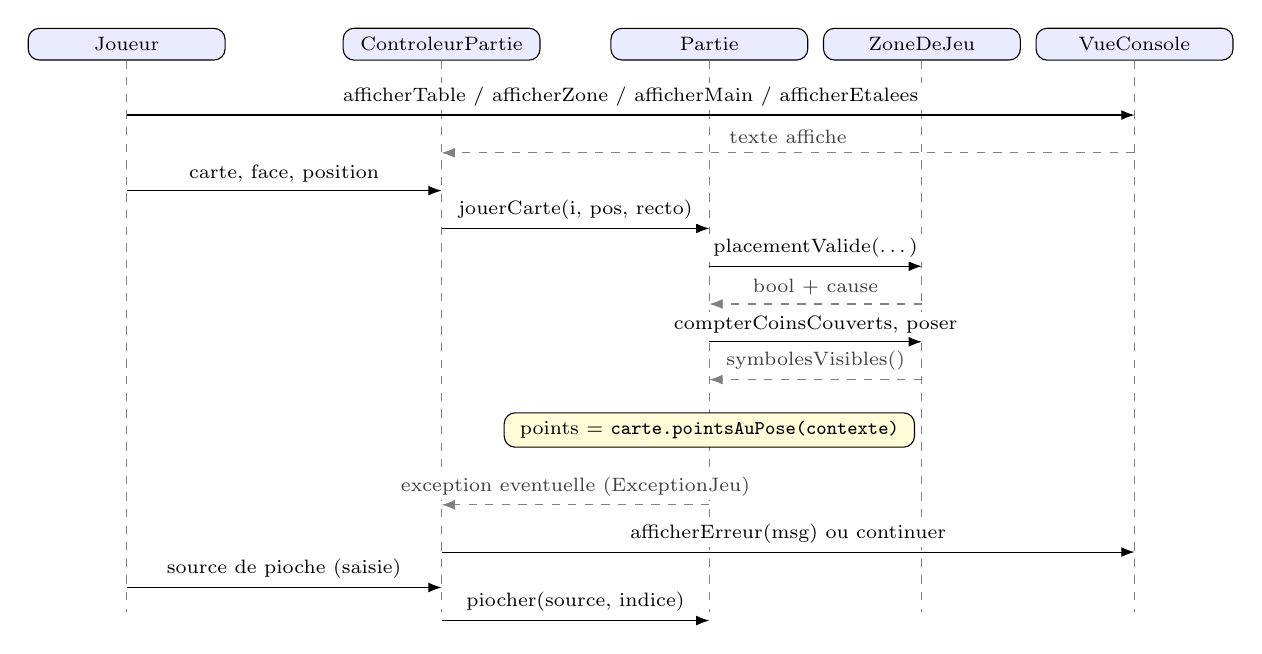
\begin{tikzpicture}[font=\scriptsize,
  part/.style={draw, rounded corners, fill=blue!8, minimum width=2.5cm, align=center},
  msg/.style={above=1.5pt, fill=white, inner sep=1.5pt, align=center},
  ret/.style={above=1.5pt, fill=white, inner sep=1.5pt, align=center, text=black!75},
  note/.style={draw, rounded corners, fill=yellow!15, align=center, inner sep=3pt}]
\node[part] (p0) at (0,0) {Joueur};
\node[part] (p1) at (4.0,0) {ControleurPartie};
\node[part] (p2) at (7.4,0) {Partie};
\node[part] (p3) at (10.1,0) {ZoneDeJeu};
\node[part] (p4) at (12.8,0) {VueConsole};
\foreach \p in {p0,p1,p2,p3,p4} {\draw[dashed, gray] (\p.south) -- ++(0,-7.0);}
\draw[-{Latex}] (p0.south |- 0,-0.90) -- node[msg] {afficherTable / afficherZone / afficherMain / afficherEtalees} (p4.south |- 0,-0.90);
\draw[-{Latex}, dashed, gray] (p4.south |- 0,-1.38) -- node[ret] {texte affiche} (p1.south |- 0,-1.38);
\draw[-{Latex}] (p0.south |- 0,-1.86) -- node[msg] {carte, face, position} (p1.south |- 0,-1.86);
\draw[-{Latex}] (p1.south |- 0,-2.34) -- node[msg] {jouerCarte(i, pos, recto)} (p2.south |- 0,-2.34);
\draw[-{Latex}] (p2.south |- 0,-2.82) -- node[msg] {placementValide(\dots)} (p3.south |- 0,-2.82);
\draw[-{Latex}, dashed, gray] (p3.south |- 0,-3.30) -- node[ret] {bool + cause} (p2.south |- 0,-3.30);
\draw[-{Latex}] (p2.south |- 0,-3.78) -- node[msg] {compterCoinsCouverts, poser} (p3.south |- 0,-3.78);
\draw[-{Latex}, dashed, gray] (p3.south |- 0,-4.26) -- node[ret] {symbolesVisibles()} (p2.south |- 0,-4.26);
\node[note, text width=5.0cm] at (7.4,-4.90) {points = \texttt{carte.pointsAuPose(contexte)}};
\draw[-{Latex}, dashed, gray] (p2.south |- 0,-5.85) -- node[ret] {exception eventuelle (ExceptionJeu)} (p1.south |- 0,-5.85);
\draw[-{Latex}] (p1.south |- 0,-6.45) -- node[msg] {afficherErreur(msg) ou continuer} (p4.south |- 0,-6.45);
\draw[-{Latex}] (p0.south |- 0,-6.90) -- node[msg] {source de pioche (saisie)} (p1.south |- 0,-6.90);
\draw[-{Latex}] (p1.south |- 0,-7.32) -- node[msg] {piocher(source, indice)} (p2.south |- 0,-7.32);
\end{tikzpicture}
\end{adjustbox}
\caption{放牌与抽牌的交互时序（虚线箭头为返回）}
\label{fig:seq}
\end{figure}

\subsection{对局状态机}
\cl{Partie} 的状态由一个枚举描述（图 \ref{fig:etats}）：
\cl{NON\_DEMARREE} $\rightarrow$ \cl{PREPARATION}（选初始牌面、选秘密目标）
$\rightarrow$ \cl{EN\_COURS} $\rightarrow$ \cl{DERNIER\_TOUR} $\rightarrow$ \cl{TERMINEE}。
\cl{DERNIER\_TOUR} 用倒计数 \cl{toursRestants} 实现「补完本轮 + 每人最后一回合」：
触发瞬间计算剩余回合数，每完成一个回合减一，归零即进入结算。

\begin{figure}[h]
\centering
\begin{adjustbox}{max width=\linewidth}
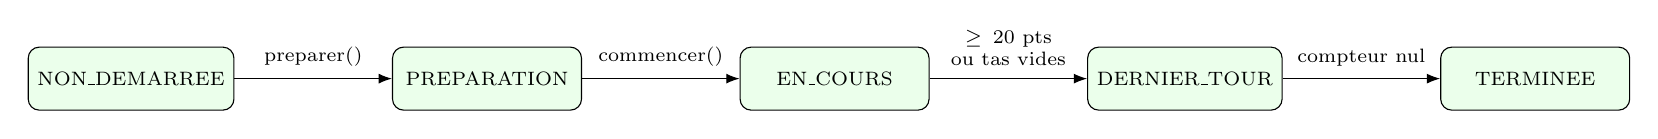
\begin{tikzpicture}[font=\scriptsize,
  etat/.style={draw, rounded corners, fill=green!8, minimum width=2.4cm,
               minimum height=8mm, align=center},
  trans/.style={above=1.2mm, font=\scriptsize, fill=white, inner sep=1pt,
                align=center, text width=1.9cm}]
\node[etat] (a) at (0,0) {NON\_DEMARREE};
\node[etat, right=20mm of a] (b) {PREPARATION};
\node[etat, right=20mm of b] (c) {EN\_COURS};
\node[etat, right=20mm of c] (d) {DERNIER\_TOUR};
\node[etat, right=20mm of d] (e) {TERMINEE};
\draw[-{Latex}] (a) -- node[trans] {preparer()} (b);
\draw[-{Latex}] (b) -- node[trans] {commencer()} (c);
\draw[-{Latex}] (c) -- node[trans] {$\ge 20$ pts ou tas vides} (d);
\draw[-{Latex}] (d) -- node[trans] {compteur nul} (e);
\end{tikzpicture}
\end{adjustbox}
\caption{对局状态机}
\label{fig:etats}
\end{figure}

\subsection{备选方案与权衡}
设计过程中比较过四种做法，最终选择都以「只用课程讲过的工具」为前提：

\begin{table}[h]
\centering
\small
\begin{tabular}{p{4.1cm}p{4.3cm}p{6.2cm}}
\toprule
问题 & 备选方案 & 采用方案与理由 \\
\midrule
如何表达「不同 AI」 & 函数指针 / 回调函数 / lambda & \textbf{Strategy 对象}：\newline 课件讲的是「用对象表示算法」，且可携带状态 \\
如何组织界面与规则 & 第三方 GUI 框架 / 事件驱动 & \textbf{抽象 \cl{Vue} + 控制台实现}：\newline 不引入外部库，模型零 I/O \\
如何保存 86 张牌 & 运行时读取 JSON/CSV & \textbf{编译期静态表}：\newline 合法使用课程内容，无需解析库，启动零依赖 \\
棋盘容器 & 变长二维数组 / 链表 & \textbf{\cl{map<Coordonnee, size\_t>}}：\newline 坐标可为负、按需增长 \\
所有权 & 裸指针 + 手动 delete & \textbf{智能指针}：\newline 异常安全，课件第 56--57 页 \\
\bottomrule
\end{tabular}
\caption{关键设计点的备选方案与最终选择}
\label{tab:choix}
\end{table}

举一个具体例子：如果允许 lambda，AI 可以写成
\cl{std::function<ActionTour(const Partie\&)>}，代码更短。但那样会同时引入
课程未讲的 lambda 与 \cl{std::function}，而且策略无法保存自己的随机数状态。
用 Strategy 基类反而更贴合课件，也让「新增 AI 不改引擎」在类型层面得到保证。

\section{类设计}

\subsection{卡牌层次（Template Method）}
\cl{Carte} 是抽象类，保存编号、所属王国与牌堆类别；\cl{face(bool)} 与 \cl{nom()} 为纯虚函数，
由 \cl{CarteRessource}、\cl{CarteDoree}、\cl{CarteInitiale} 实现。
计分采用模板方法：骨架「固定分 + 可变分」只写一次，变化点留给子类。

\begin{lstlisting}
class Carte {
public:
    int pointsAuPose(const ContextePose& contexte) const {
        return pointsFixes() + pointsVariables(contexte);   // trame fixe
    }
    virtual bool exigencesSatisfaites(const std::map<Ressource,int>&) const;
protected:
    virtual int pointsFixes() const = 0;                    // etape 1
    virtual int pointsVariables(const ContextePose&) const; // etape 2 (hook, 0 par defaut)
};
\end{lstlisting}

\cl{CarteRessource} 只实现第一步（0 或 1 分）；\cl{CarteDoree} 实现两步
（固定分 / 每覆盖角 2 分 / 每物件 1 分）并实现资源需求判断；
\cl{CarteInitiale} 得 0 分。新增一类牌时只需新增子类与数据表条目，引擎无需修改。

\begin{figure}[h]
\centering
\begin{adjustbox}{max width=\linewidth}
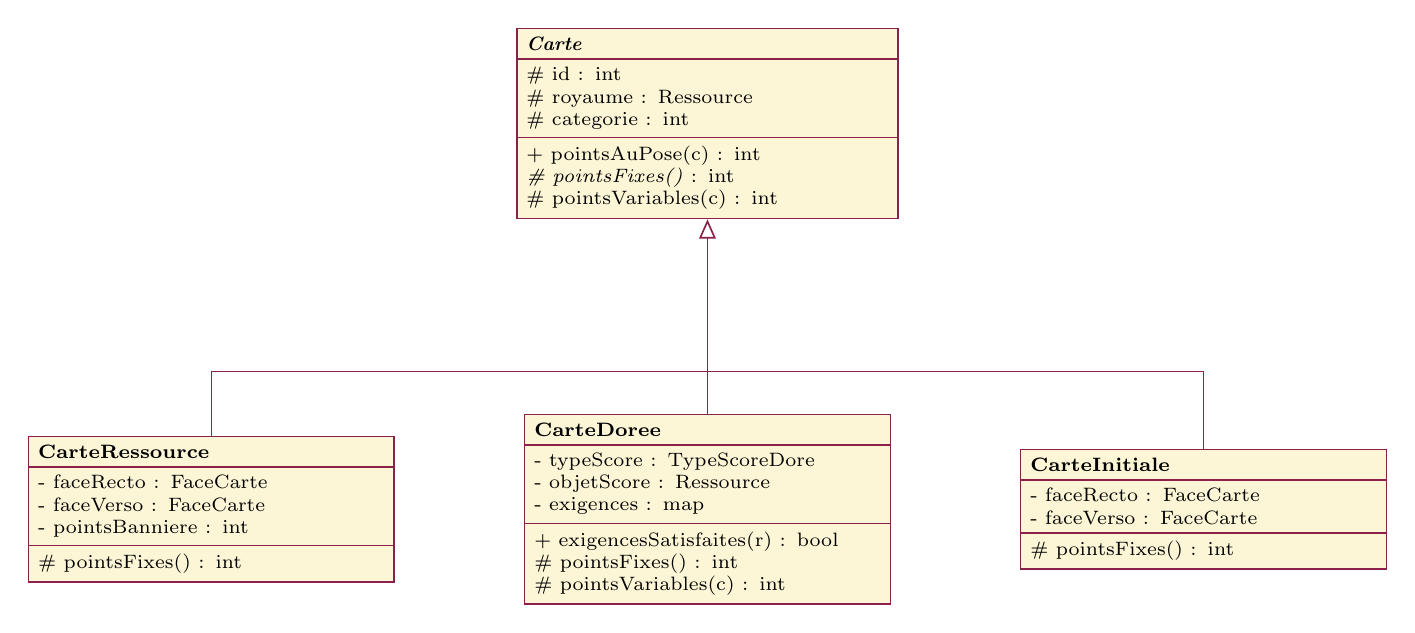
\begin{tikzpicture}
\umlbox{Carte}{\textit{Carte}}{0,0}{4.6cm}{%
  \# id : int\\
  \# royaume : Ressource\\
  \# categorie : int}{%
  + pointsAuPose(c) : int\\
  \textit{\# pointsFixes()} : int\\
  \# pointsVariables(c) : int}
\umlbox{CarteRessource}{CarteRessource}{-6.3,-4.9}{4.4cm}{%
  - faceRecto : FaceCarte\\
  - faceVerso : FaceCarte\\
  - pointsBanniere : int}{%
  \# pointsFixes() : int}
\umlbox{CarteDoree}{CarteDoree}{0,-4.9}{4.4cm}{%
  - typeScore : TypeScoreDore\\
  - objetScore : Ressource\\
  - exigences : map}{%
  + exigencesSatisfaites(r) : bool\\
  \# pointsFixes() : int\\
  \# pointsVariables(c) : int}
\umlbox{CarteInitiale}{CarteInitiale}{6.3,-4.9}{4.4cm}{%
  - faceRecto : FaceCarte\\
  - faceVerso : FaceCarte}{%
  \# pointsFixes() : int}
% generalisation : les trois sous-classes partagent une pointe unique
\coordinate (busC) at (0,-3.15);
\foreach \c in {CarteRessource, CarteDoree, CarteInitiale} {
  \draw[umlline] (\c.north) -- (\c.north |- busC);
}
\draw[umlline] (CarteRessource.north |- busC) -- (CarteInitiale.north |- busC);
\draw[umlgen] (busC) -- (Carte.south);
\end{tikzpicture}
\end{adjustbox}
\caption{\cl{Carte} 层次（斜体为纯虚函数）}
\label{fig:carte}
\end{figure}

\subsection{目标层次（Composite）}
目标抽象类 \cl{Objectif} 只有两个操作：\cl{evaluer(const ZoneDeJeu\&)} 与
\cl{description()}。四个具体子类分别实现斜线/L 型、三同资源、物件对、物件三异。
\cl{ObjectifCompose} 持有一组子目标并递归求和——这正是组合模式：
调用方无法也不需要区分「单个条件」与「条件组合」。

\begin{figure}[h]
\centering
\begin{adjustbox}{max width=\linewidth}
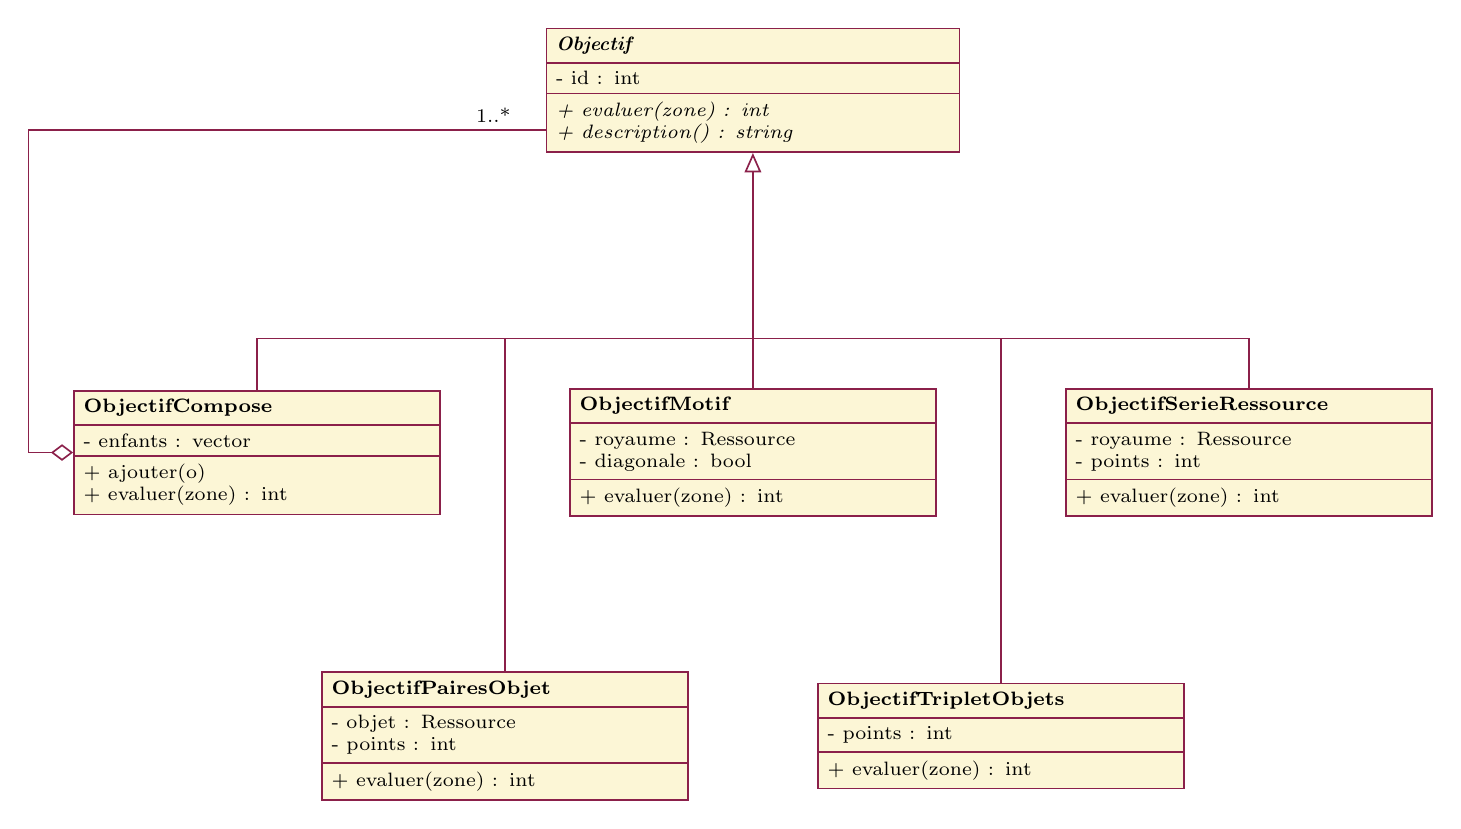
\begin{tikzpicture}
\umlbox{Objectif}{\textit{Objectif}}{0,0}{5.0cm}{%
  - id : int}{%
  \textit{+ evaluer(zone) : int}\\
  \textit{+ description() : string}}
\umlbox{ObjectifCompose}{ObjectifCompose}{-6.3,-4.6}{4.4cm}{%
  - enfants : vector}{%
  + ajouter(o)\\
  + evaluer(zone) : int}
\umlbox{ObjectifMotif}{ObjectifMotif}{0,-4.6}{4.4cm}{%
  - royaume : Ressource\\
  - diagonale : bool}{%
  + evaluer(zone) : int}
\umlbox{ObjectifSerieRessource}{ObjectifSerieRessource}{6.3,-4.6}{4.4cm}{%
  - royaume : Ressource\\
  - points : int}{%
  + evaluer(zone) : int}
\umlbox{ObjectifPairesObjet}{ObjectifPairesObjet}{-3.15,-8.2}{4.4cm}{%
  - objet : Ressource\\
  - points : int}{%
  + evaluer(zone) : int}
\umlbox{ObjectifTripletObjets}{ObjectifTripletObjets}{3.15,-8.2}{4.4cm}{%
  - points : int}{%
  + evaluer(zone) : int}
% generalisation : les cinq sous-classes partagent une pointe unique
\coordinate (busO) at (0,-3.15);
\foreach \c in {ObjectifCompose, ObjectifMotif, ObjectifSerieRessource,
                ObjectifPairesObjet, ObjectifTripletObjets} {
  \draw[umlline] (\c.north) -- (\c.north |- busO);
}
\draw[umlline] (ObjectifCompose.north |- busO) -- (ObjectifSerieRessource.north |- busO);
\draw[umlgen] (busO) -- (Objectif.south);
% composition : le tout (ObjectifCompose) porte 1..* parties (Objectif)
\coordinate (ow) at ([yshift=-0.5cm]Objectif.west);
\draw[umlagg] (ObjectifCompose.west)
  -- (-9.2,0 |- ObjectifCompose.west) -- (-9.2,0 |- ow) -- (ow);
\node[umlmult, above left] at ([xshift=-0.4cm,yshift=1.5pt]ow) {1..*};
\end{tikzpicture}
\end{adjustbox}
\caption{目标层次：\cl{ObjectifCompose} 聚合（空心菱形）1..* 个 \cl{Objectif}，另有四个叶子子类}
\label{fig:objectif}
\end{figure}

\subsection{棋盘、牌堆与玩家}
\cl{ZoneDeJeu} 内部有两份数据：\cl{std::map<Coordonnee, std::size\_t> grille}
记录「每个格子属于第几张牌」，\cl{std::vector<CartePlacee> liste} 记录已放牌
（左上角坐标、牌对象、正反面、覆盖了几个角）。一张牌的四个角就是它的四个格子；
某个角「可见」当且仅当该格仍属于这张牌。三条规则由此自然成立：
\begin{itemize}
\item 只能放在已有牌的\textbf{对角}相邻格，否则会同时覆盖两张牌的两个角，非法；
\item 「缺失角」（\cl{CACHE}）永远不能覆盖；
\item 每次放牌后资源自动重算，因此「盖上资源」的代价自然出现。
\end{itemize}
\cl{Pioche} 管理两个牌堆与 4 张明牌（2 资源 + 2 镀金），并提供
\cl{prendreEtalee} / \cl{piocherSurLeTas} / \cl{completerEtalees}。
\cl{Joueur} 持有自己的区域、手牌、秘密目标与分数；\cl{Partie} 持有玩家数组、牌堆、
2 张公共目标与回合状态。玩家数组与区域按值存放，故下图为\textbf{组合}（实心菱形）；
\cl{ObjectifCompose} 的子目标由 \cl{shared\_ptr} 共享，故图~\ref{fig:objectif} 为聚合（空心菱形）。

\begin{figure}[h]
\centering
\begin{adjustbox}{max width=\linewidth}
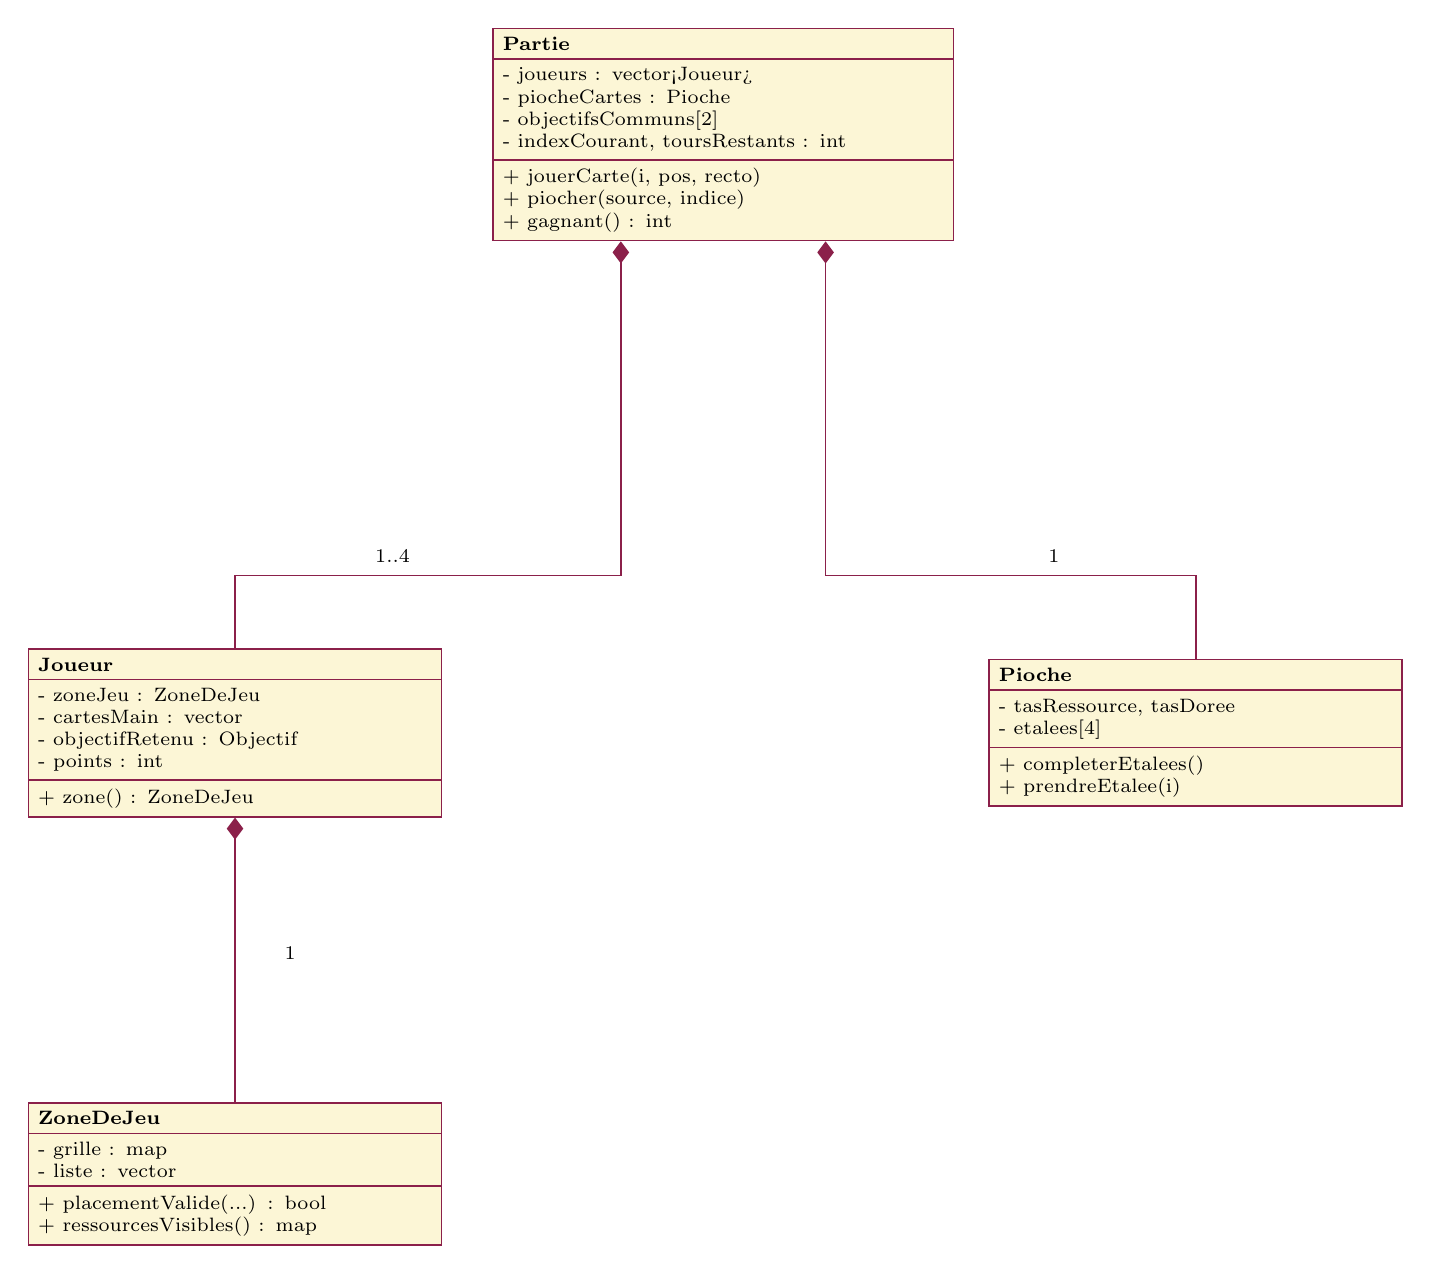
\begin{tikzpicture}
\umlbox{Partie}{Partie}{0,0}{5.6cm}{%
  - joueurs : vector<Joueur>\\
  - piocheCartes : Pioche\\
  - objectifsCommuns[2]\\
  - indexCourant, toursRestants : int}{%
  + jouerCarte(i, pos, recto)\\
  + piocher(source, indice)\\
  + gagnant() : int}
\umlbox{Joueur}{Joueur}{-6.2,-7.6}{5.0cm}{%
  - zoneJeu : ZoneDeJeu\\
  - cartesMain : vector\\
  - objectifRetenu : Objectif\\
  - points : int}{%
  + zone() : ZoneDeJeu}
\umlbox{Pioche}{Pioche}{6.0,-7.6}{5.0cm}{%
  - tasRessource, tasDoree\\
  - etalees[4]}{%
  + completerEtalees()\\
  + prendreEtalee(i)}
\umlbox{ZoneDeJeu}{ZoneDeJeu}{-6.2,-13.2}{5.0cm}{%
  - grille : map\\
  - liste : vector}{%
  + placementValide(...) : bool\\
  + ressourcesVisibles() : map}
% composition : les parties sont detruites avec le tout
\coordinate (pJ) at ([xshift=-1.3cm]Partie.south);
\coordinate (pP) at ([xshift=1.3cm]Partie.south);
\draw[umlcomp] (pJ) -- (pJ |- 0,-5.6) -- (-6.2,-5.6) -- (Joueur.north);
\draw[umlcomp] (pP) -- (pP |- 0,-5.6) -- (6.0,-5.6) -- (Pioche.north);
\draw[umlcomp] (Joueur.south) -- (ZoneDeJeu.north);
\node[umlmult] at (-4.2,-5.35) {1..4};
\node[umlmult] at (4.2,-5.35) {1};
\node[umlmult] at (-5.5,-10.4) {1};
\end{tikzpicture}
\end{adjustbox}
\caption{引擎核心：\cl{Partie} 组合 1..4 个 \cl{Joueur} 与 1 副 \cl{Pioche}，\cl{Joueur} 组合 1 个 \cl{ZoneDeJeu}}
\label{fig:engine}
\end{figure}

\newpage
\subsection{卡表与编码}
卡表以 C++ 静态数组形式编入（\cl{src/modele/DonneesCartes.cpp}），运行时不读任何文件，
因此不需要 JSON 解析库。每条记录描述一张牌：

\begin{lstlisting}
struct DonneeCarte {
    int id;                    // 1..40 ressource, 41..80 doree, 81..86 initiale
    Ressource royaume;         // royaume de la carte
    int categorie;             // CATEGORIE_RESSOURCE / DOREE / INITIALE
    DonneeFace recto, verso;   // 4 coins + 0..3 ressources permanentes
    int score;                 // points de banniere
    TypeScoreDore typeScore;   // AUCUN / STATIQUE / PAR_ANGLE / PAR_OBJET
    Ressource objetScore;      // objet compte pour PAR_OBJET
    int exigences[4];          // nombre exige de chaque royaume
};
\end{lstlisting}

角上的符号用字符编码：P 植物、A 动物、C 真菌、I 昆虫、f 羽毛、j 墨水瓶、s 羊皮纸、
点号表示可见空角、井号表示缺失角。测试 \cl{tests/test\_cartes.cpp} 用 14 条断言核对整张表：
86 张牌、16 个目标、每王国 10 张资源牌、12 张 1 分资源牌、16 张固定分镀金牌、
12 张按角、12 张按物件。

\subsection{代码规模与文件职责}
\begin{table}[h]
\centering
\small
\begin{tabular}{p{2.8cm}p{3.0cm}p{8.2cm}}
\toprule
目录 & 规模 & 职责 \\
\midrule
\cl{src/noyau} & 11 文件 / 302 行 & 资源枚举与符号、坐标、随机数、异常层次、洗牌模板 \\
\cl{src/modele} & 36 文件 / 2706 行 & 卡牌与目标层次、棋盘、牌堆、玩家、引擎、卡表、AI \\
\cl{src/vue} & 4 文件 / 312 行 & \cl{Vue} 接口与控制台实现 \\
\cl{src/controleur} & 10 文件 / 623 行 & 菜单、主循环、输入适配、自动回合、批量模拟 \\
\cl{src/main.cpp} & 126 行 & 命令行参数与模式选择 \\
\cl{tests} & 8 文件 / 534 行 & 断言宏、测试工具、五个测试文件 \\
\midrule
合计 & 70 文件 / 4603 行 & 源码 4069 行 + 测试 534 行 \\
\bottomrule
\end{tabular}
\caption{代码规模与各目录职责}
\label{tab:taille}
\end{table}
模型层占比约三分之二，符合「规则是项目的核心」这一判断；
界面与控制层加起来不到四分之一，说明业务逻辑没有被界面代码淹没。

\section{设计模式的应用}
表 \ref{tab:patterns} 汇总七个模式的落点，随后逐条说明收益。

\begin{table}[h]
\centering
\small
\begin{tabular}{p{2.8cm}p{5.6cm}p{6.4cm}}
\toprule
模式 & 本项目中的类 & 解决的问题 \\
\midrule
Template Method & \cl{Carte::pointsAuPose}、\cl{VueConsole} 的渲染骨架 & 固定算法骨架，变化点下放子类 \\
Strategy & \cl{StrategieIA}：\cl{IAHasard}、\cl{IAGloutonne}、\cl{IAObjectifs} & 运行期切换 AI 算法，新增 AI 不改引擎 \\
Factory Method & \cl{FabriqueCartes}（3 个子类）\newline \cl{FabriqueObjectif}（5 个子类） & 创建与使用分离 \\
Singleton & \cl{CatalogueCartes} & 全应用唯一只读卡库 \\
Iterator & \cl{IterateurCartes} & 不暴露内部结构即可遍历棋盘 \\
Adapter & \cl{AdaptateurFlux} & 同一控制器读键盘或读脚本文件 \\
Composite & \cl{Objectif} / \cl{ObjectifCompose} & 单条件与条件组合统一处理 \\
\bottomrule
\end{tabular}
\caption{七个设计模式在本项目中的落点}
\label{tab:patterns}
\end{table}

\subsection{Template Method：计分与显示}
计分骨架（取固定分 $\rightarrow$ 加上可变分）只在 \cl{Carte::pointsAuPose} 写一次。
镀金牌的三种计分方式（固定、按角、按物件）都只是重写 \cl{pointsVariables}；
资源牌只重写 \cl{pointsFixes}。显示层同样使用模板方法：\cl{VueConsole::afficherZone}
固定执行「标题 $\rightarrow$ 角标网格 $\rightarrow$ 已放牌清单 $\rightarrow$ 资源统计」，
子步骤由私有函数实现，将来换成图形界面只需实现 \cl{Vue} 接口。

\subsection{Strategy：三种 AI}
\cl{StrategieIA} 声明唯一的操作 \cl{choisirAction(const Partie\&, int)}，三个子类分别是：
\begin{itemize}
\item \cl{IAHasard}：在所有合法落点中随机选一个，抽牌也随机；
\item \cl{IAGloutonne}：逐张牌、逐面、逐落点模拟，取「即时分 $\times 10$ + 资源种类数」最大者；
\item \cl{IAObjectifs}：在贪心基础上再加上「目标增益 $\times 6$」与「同王国邻接数 $\times 3$」，
      因此会主动为斜线/L 图案铺路。
\end{itemize}
\cl{Partie} 只持有 \cl{std::shared\_ptr<StrategieIA>}，换 AI 只是换对象；
这正是课件所说「用对象表示算法」的做法，本项目没有使用 lambda 或函数指针。

\subsection{Factory Method 与 Singleton}
\cl{FabriqueCartes} 有三个子类，分别生产资源牌、镀金牌、初始牌；
\cl{FabriqueObjectif} 有五个子类，每个负责一种目标卡。目录类
\cl{CatalogueCartes} 是单例：私有构造、静态指针、\cl{instance()} 首次调用时创建，
内部持有 \cl{map<int, shared\_ptr<const Carte>>} 与 \cl{map<int, shared\_ptr<const Objectif>>}，
并对外提供 \cl{creerCarte(id)}、\cl{creerObjectif(id)} 这样的参数化工厂方法。
单例的写法与课件第 104 页一致（\cl{donneInstance()}、私有构造、静态指针）。

\subsection{Iterator 与 Adapter}
\cl{IterateurCartes} 提供 \cl{premier/estFini/courant/suivant} 四个操作，
显示层与目标计算都通过它遍历棋盘，不需要知道内部使用的是 \cl{map} 还是别的容器。
\cl{AdaptateurFlux} 把 \cl{std::istream} 适配成 \cl{Saisie} 接口，于是同一份
\cl{ControleurPartie} 既能读键盘，也能重放 \cl{scripts/demo\_entree.txt} 中的脚本——
演示视频的「确定性演示」和自动化测试都依赖它。

\subsection{Composite}
一张目标卡可能同时包含多个图案条件。\cl{ObjectifCompose} 持有一组
\cl{shared\_ptr<const Objectif>}，\cl{evaluer} 递归求和；
调用方对单个条件与组合条件一视同仁，新增「复合目标卡」不需要改结算代码。

\section{关键算法}

\subsection{放置合法性}
给定新牌、目标格 $(x,y)$ 与正反面，算法如下：
\begin{enumerate}
\item 对四个格子：若已被占用，找到其主人与对应角；若该角是缺失角，拒绝；
\item 若四个格子全部为空，拒绝（必须覆盖至少一个可见角）；
\item 若同一张牌被覆盖两个角，拒绝（在 $2\times2$ 模型下这等价于正交相邻）；
\item 若为镀金牌且玩的是正面：检查场上可见资源是否满足需求。
\end{enumerate}
伪代码：
\begin{lstlisting}
bool placementValide(pos, carte, recto) const {
    int representants = 0;
    std::map<size_t,int> coinsParCarte;
    for (int coin = 0; coin < 4; ++coin) {
        Coordonnee c = caseDuCoin(pos, coin);
        if (caseLibre(c)) continue;
        ++representants;
        const CartePlacee& autre = *carteSur(c);
        int coinTouche = coinDepuisDecalage(c.x - autre.origine.x, c.y - autre.origine.y);
        if (!coinUtilisable(autre.carte->face(autre.recto).coin(coinTouche))) return false;
        ++coinsParCarte[indice(autre)];
    }
    if (representants == 0) return false;
    // aucun doublon de carte + exigences de la carte doree
}
\end{lstlisting}

\subsection{可见资源与物件}
遍历已放牌：对每个角，若该格仍属于这张牌则计入符号；再加上该面的中央永久资源。
镀金牌「每物件 1 分」必须在放牌瞬间结算一次，之后不再重算——这一点由
\cl{ContextePose} 的快照实现：\cl{Partie} 在放牌后立刻调用
\cl{symbolesVisibles()} 并把结果放进 \cl{ContextePose} 传给 \cl{pointsAuPose}。

\subsection{目标计分}
斜线与 L 型是\textbf{几何}目标：把同王国牌的左上角坐标放进 \cl{std::set}，
按「从上到下、从左到右」的固定顺序贪心取不重叠的三元组；斜线有两个方向，
L 型由「两个互相垂直的对角步」构成（4 个方向）。贪心保证确定性与「每张牌只用一次」。
三同资源、物件对、物件三异是\textbf{计数}目标：统计可见符号数后做整除。
两个公共目标与秘密目标分别计算，最后相加。

\subsection{AI 决策}
候选动作数为「手牌数 $\times$ 2 面 $\times$ 候选格数」，候选格数约为已放牌数的 4 倍
（每张牌四个对角格），因此单次决策在毫秒级。评分函数见表 \ref{tab:ia}。
为避免偷看信息，AI 只读取公有接口：自己的手牌、所有可见区域、公共目标与自己持有的秘密目标。

\begin{table}[h]
\centering
\small
\begin{tabular}{p{3.2cm}p{9.6cm}}
\toprule
AI & 评分函数（越大越好） \\
\midrule
\cl{IAHasard} & 均匀随机取一个合法动作 \\
\cl{IAGloutonne} & $10 \times$ 即时分 $+$ 资源种类数 \\
\cl{IAObjectifs} & $10 \times$ 即时分 $+ 6 \times$ 目标增益 $+ 2 \times$ 资源种类数 $+ 3 \times$ 同王国对角邻接数 \\
抽牌策略 & 评估 4 张明牌（镀金牌基础分更高、角上资源更多者优先），否则从资源/镀金堆抽取 \\
\bottomrule
\end{tabular}
\caption{三种 AI 的评分函数}
\label{tab:ia}
\end{table}

\subsection{终局与平局}
触发条件：任意玩家分数 $\ge 20$，或两个牌堆都空。触发后引擎计算
\cl{toursRestants = (本轮剩余玩家) + 玩家人数}，每完成一个回合减一，归零即结算。
结算依次计算：牌面分（已累计）、公共目标 1、公共目标 2、秘密目标，得到总分；
比较顺序为总分 $\rightarrow$ 目标分 $\rightarrow$ 并列。
另外，若某玩家手上已无合法落点，引擎允许其「弃权」；连续弃权达到人数时提前结束，
以避免死循环。

\subsection{复杂度与性能}
\begin{table}[h]
\centering
\small
\begin{tabular}{p{4.6cm}p{4.6cm}p{4.2cm}}
\toprule
操作 & 复杂度 & 说明 \\
\midrule
一次放置校验 & $O(1)$ & 只看四个格子 \\
可见资源重算 & $O(n)$ & $n$ 为已放牌数（最多约 40） \\
目标计分 & $O(n \log n)$ & 排序 + 贪心取三元组 \\
AI 决策 & $O(n \cdot k \cdot 2 \cdot 4n)$ & $k$ 为手牌数（3） \\
200 局自动对局 & 约 7 秒 & 4 名最高难度 AI \\
\bottomrule
\end{tabular}
\caption{关键操作复杂度与实测性能}
\label{tab:perf}
\end{table}

\subsection{异常与错误处理}
模型层用异常表达「动作被拒绝」，控制器是唯一捕获它们的地方：
捕获后显示原因并让玩家重新输入，对局状态不变（校验全部在修改之前完成）。
异常层次如下：

\begin{table}[h]
\centering
\small
\begin{tabular}{p{4.5cm}p{2.9cm}p{7.2cm}}
\toprule
异常类 & 典型触发 & 面向玩家的消息（示例） \\
\midrule
\cl{PlacementInvalide} & 落点非法 & la carte doit recouvrir au moins un coin visible \\
 &  & la carte recouvrirait deux coins de la meme carte \\
 &  & le coin vise par la carte R17 est cache \\
\cl{RessourcesInsuffisantes} & 镀金资源不足 & D55 : exige 3 plante 1 animal \\
\cl{CarteAbsente} & 手牌下标非法、明牌已被取走 & indice de carte en main invalide \\
\cl{SaisieInvalide} & 输入不是数字或越界 & ce n'est pas un nombre : abc \\
\cl{PartieTerminee} & 终局后继续操作 & la partie est terminee \\
\cl{IdentifiantInconnu} & 卡表/目标 id 不存在 & carte inconnue : 999 \\
\bottomrule
\end{tabular}
\caption{异常层次与典型消息}
\label{tab:exceptions}
\end{table}

值得强调的是「异常安全」：\cl{Partie::jouerCarte} 先完成全部校验（放置规则、资源需求、
手牌范围），只有全部通过后才修改分数、手牌和棋盘。因此任何一次被拒绝的动作都不会留下
「扣了牌却没放上去」这类半完成状态——这也是为什么测试可以直接反复尝试非法输入。

\section{可扩展性论证}

\subsection{新增一个 AI}
\begin{lstlisting}
class IAExperte : public StrategieIA {
public:
    explicit IAExperte(GenerateurAleatoire& g) : generateur(&g) {}
    ActionTour choisirAction(const Partie& partie, int indice) { /* ... */ }
    std::string nom() const { return "IA experte"; }
private:
    GenerateurAleatoire* generateur;
};
// dans creerStrategie(int niveau, ...) : un test de plus, une ligne
\end{lstlisting}
\textbf{不改}：\cl{Partie}、\cl{Joueur}、\cl{ZoneDeJeu}、\cl{VueConsole}、控制器。

\subsection{新增一种目标卡}
新增 \cl{ObjectifMotifCroix : Objectif} 与 \cl{FabriqueObjectifCroix : FabriqueObjectif}，
在 \cl{CatalogueCartes} 构造函数里多注册一个 \cl{TypeObjectif::CROIX} 分支，
数据表里多两行。\textbf{不改}结算代码，因为 \cl{Partie::pointsObjectifs} 只调用
\cl{Objectif::evaluer}。

\subsection{新增一类牌}
例如扩展「灵魂牌」：新增 \cl{CarteEsprit : Carte} 与对应 \cl{FabriqueCarteEsprit}，
在 \cl{DonneesCartes.h} 里加一个 \cl{CATEGORIE\_ESPRIT} 常量，数据表加若干条。
\textbf{不改}：计分（模板方法自动复用）、放置规则、显示（都是对 \cl{Carte} 抽象操作）。

\subsection{新增一种显示方式}
实现 \cl{Vue} 接口（例如彩色终端界面或图形界面），在 \cl{main} 里替换对象。
\textbf{不改}模型层任何代码。

\subsection{接入官方单人模式（Tybor）}
官方单人模式使用专属卡组与计分表。做法：新增 \cl{StrategieTybor : StrategieIA} 与一份
单人卡组数据；\cl{Partie} 的回合、放置、计分流程完全复用。这正是作业要求
「架构易于整合新组件、新 AI」的直接体现。

\begin{table}[h]
\centering
\small
\begin{tabular}{p{2.8cm}p{6.2cm}p{5.2cm}}
\toprule
扩展 & 需要新增 & 需要修改的既有代码 \\
\midrule
新 AI & \cl{IAExperte}（实现 \cl{StrategieIA}） & \cl{creerStrategie} 加一行 \\
新目标类型 & \cl{ObjectifX} + \cl{FabriqueObjectifX} & 目录注册一行 \\
新牌类 & \cl{CarteX} + 数据表条目 & 无 \\
新显示 & \cl{VueGraphique : Vue} & \cl{main} 换一个对象 \\
官方单人模式 & \cl{StrategieTybor} + 单人卡组数据 & 无 \\
存档 / 悔棋 & \cl{Memento} 类（未实现） & \cl{Partie} 增加保存/恢复接口 \\
\bottomrule
\end{tabular}
\caption{扩展场景与改动范围}
\label{tab:extensions}
\end{table}

\section{项目计划与实际执行}

\subsection{任务分解与排期}
\begin{table}[h]
\centering
\small
\begin{tabular}{p{2.0cm}p{7.0cm}p{2.5cm}p{2.2cm}}
\toprule
周次 & 任务 & 依赖 & 状态 \\
\midrule
第 1--2 周 & 读规则、试玩、整理 86 张牌的数据表与计分规则 & --- & 完成 \\
第 3 周 & 架构设计：分层、模式选型、UML 草图、接口定稿 & 数据表 & 完成 \\
第 4 周 & \cl{noyau} + 卡牌层次 + 单例目录 + 工厂 & 架构 & 完成 \\
第 5 周 & 棋盘几何、放置校验、可见资源与物件 & 卡牌 & 完成 \\
第 6 周 & 目标计分、终局判定、单元测试骨架 & 棋盘 & 完成 \\
第 7 周 & 控制台界面、控制器、脚本演示、三种 AI & 引擎 & 完成 \\
第 8 周 & 报告、UML 图、视频、打包与提交 & 全部 & 完成 \\
\bottomrule
\end{tabular}
\caption{计划与实际执行}
\label{tab:planning}
\end{table}


\subsection{风险与应对}
\begin{itemize}
\item \textbf{规则歧义}：目标卡的图案方向在原版图示中不完全清晰。应对：按「两次垂直对角步」
      实现 L 型，并把解释写入 \cl{docs/REGLES\_OBJECTIFS.md}；若需调整，只需新增一个
      \cl{Objectif} 子类。
\item \textbf{中文排版}：报告用 XeLaTeX + ctex，先做最小样例验证字体与 UML 宏包可用，
      再正式撰写，避免最后一天才发现编译问题。
\item \textbf{过度设计}：课程讲了十余个模式，本项目只保留真正被用到的七个，
      「不加功能就不加类」。
\item \textbf{死循环}：曾有「所有玩家都无合法落点」导致对局无法结束的问题；
      加入连续弃权计数与轮次上限后消除。
\end{itemize}

\subsection{回顾}
实际执行比计划多花了两天，主要用在两处：一是把「$2\times2$ 格子」的几何模型推清楚
（包括 L 型图案该如何在斜格上定义），二是把 \cl{Partie} 的异常安全语义做扎实
（校验全部前置，失败不修改状态）。这两处投入在后期写测试时得到了回报。

\Needspace{14\baselineskip}
\section{个人分工与工作量}
\begin{table}[h]
\centering
\small
\setlength{\tabcolsep}{4.5pt}
\begin{tabular}{p{2.2cm}p{7.3cm}p{3.9cm}p{1.8cm}}
\toprule
成员 & 主要负责部分 & 交付物 & 贡献占比 \\
\midrule
袁鹏杰 & 86 张卡的静态数据表与一致性校验；\cl{Carte} 四层继承层次与模板方法计分；
         卡牌工厂与单例卡表 & 代码、数据核对、视频 & 30\% \\
刘羽骋 & 稀疏网格棋盘模型（\cl{map}，支持负坐标与按需增长）；放置合法性四类判定
         （可见角、隐藏角、重叠、镀金资源需求）；四角覆盖计数与可见资源统计 & 代码、单元测试 & 30\% \\
张浩冉 & 五类目标计分；终局补轮与最终一回合结算；三种 AI 难度策略 & 代码、测试 & 13\% \\
梁皓 & 控制台视图与输入解析；回合控制流、自动对局与演示输入脚本 & 代码、演示脚本 & 13\% \\
王蕊 & 架构与规则文档；报告排版与 UML 图 & 报告 & 13\% \\
\midrule
合计 & \strut & \strut & 99\% \\
\bottomrule
\end{tabular}
\caption{分工与贡献占比}
\label{tab:contrib}
\end{table}

\section{测试与验证}

\subsection{测试方法}
不引入第三方框架：\cl{tests/harnais.h} 用三个宏（相等、为真、抛异常）实现断言，
按模块划分为 5 个文件（卡表、棋盘、目标、引擎、AI）。运行方式：
\begin{center}
\begin{minipage}{\linewidth}
\begin{lstlisting}
powershell -ExecutionPolicy Bypass -File scripts\build.ps1
#   Compilation du jeu... / Compilation des tests... / Execution des tests...
#   207 verifications, 0 echec(s).   TOUS LES TESTS PASSENT
powershell -ExecutionPolicy Bypass -File scripts\check_scope.ps1
#   Aucune fonctionnalite hors cours detectee
\end{lstlisting}
\end{minipage}
\end{center}

\Needspace{17\baselineskip}
\subsection{测试明细}
\begin{longtable}{p{3.9cm}p{2.6cm}p{7.3cm}}
\toprule
测试文件 & 断言数 & 覆盖内容 \\
\midrule
\cl{test\_cartes.cpp} & 14 & 86 张牌、16 目标、每王国 10 张、12 张 1 分、16/12/12 三类镀金、非法 id 抛异常 \\
\cl{test\_zone.cpp} & 13 & 空区、对角放置、隔离放置拒绝、缺失角拒绝、重叠拒绝、双角覆盖合法、覆盖后资源减少、迭代器计数 \\
\cl{test\_objectifs.cpp} & 12 & 斜线、L、混合王国无效、三同资源、物件对、三异、组合目标求和 \\
\cl{test\_partie.cpp} & 12 & 开局手牌、准备阶段不可放牌、先放后抽、终局、总分 = 牌面 + 目标、胜者合法 \\
\cl{test\_ia.cpp} & 12 局 & 1--4 人 $\times$ 3 难度完整对局，分数与总量一致性 \\
\midrule
合计 & 207 次断言 & 见上 \\
\bottomrule
\caption{单元与集成测试明细}
\label{tab:tests}
\end{longtable}

\subsection{稳定性与可复现性}
\cl{GenerateurAleatoire} 是自写的线性同余发生器（不使用随机设备），
因此「同一种子 $\Rightarrow$ 同一局」完全成立。批量验证：
\begin{lstlisting}
codex_naturalis --auto 200 --joueurs 4 --niveau 3 --graine 2026
# 200 partie(s) terminee(s), environ 6200 tours joues, aucune exception
\end{lstlisting}
工程层面还做了两项检查：全部源文件在 \cl{-std=c++14} 与 \cl{-std=c++17} 下编译，
并开启 \cl{-Wall -Wextra -pedantic}，结果均为零警告。

\section{界面流程与使用体验}
题目允许只用控制台，但要求「画面足以看懂局面」。本项目的界面分三个环节，
每一步都只用文本表格与固定列宽（\cl{iomanip}），不依赖颜色或终端控制字符。

\subsection{开局}
\cl{Menu} 依次询问人数（1--4）、每个座位的姓名、真人或电脑（以及电脑难度）、随机种子。
随后进入准备阶段，逐位玩家显示自己的初始牌正反两面（四个角的符号与中央永久资源），
再显示两张候选秘密目标的文字描述，让玩家二选一。这些询问都可以用一个文本文件重放
（\cl{--entree}），因此同一场演示可以精确复现。

\subsection{回合}
每次轮到真人玩家时，界面按固定顺序打印四块信息：
\begin{enumerate}
\item 局面：所有玩家分数、两个牌堆剩余张数、当前玩家、当前该做什么（放牌还是抽牌）；
\item 自己的手稿：以坐标网格显示的角标矩阵（每个格一个符号），后面跟「已放牌清单」
      （每张牌的编号、位置、正反面、四角符号、中央资源、覆盖了几个角）；
\item 自己的手牌：每张牌的正反面符号与需求说明；
\item 桌面中央的 4 张明牌。
\end{enumerate}
然后程序只列出\textbf{当前合法}的落点（编号 + 坐标），玩家输入编号即可，无需自己算坐标。
若输入非法（例如手牌编号越界、或者该牌此刻无法放置），程序给出原因并重新询问，
不会中断对局。

\subsection{终局}
触发终局后先打印最后几回合的提示，再输出结果表：每位玩家的「牌面分 / 目标分 / 总分」，
最后一行给出胜者或「平局」。若总分相同则按目标分比较，这一点在结果表里可以直接看出来。

\subsection{可读性取舍}
做过两个取舍：其一，\textbf{不画牌的美术图案}，只画四个角与中央资源，
因为「能不能放、能拿几分」完全由这些符号决定；其二，\textbf{不隐藏信息}，
所有区域与手牌都完整显示，因为本地同一台机器对战没有信息隐藏的必要。
这两点都在 \cl{docs/REGLES\_OBJECTIFS.md} 中记录为「有意为之的简化」。

\section{结论与展望}
本项目用课程所讲的 C++ 完成了 Codex Naturalis 的完整实现：规则正确、博弈完整、
可复现、可扩展。三个最关键的设计决定是：
（1）模型层零输入输出，使引擎可被脚本与测试直接驱动；
（2）依赖抽象类型（\cl{Carte}、\cl{Objectif}、\cl{StrategieIA}、\cl{Vue}），
使扩展只需新增子类；
（3）用数据表 + 工厂把「86 张牌」与「规则代码」彻底分离。
后续可以继续做：官方单人 Tybor 模式、图形界面、存档（Memento）、
以及更多扩展牌与新的目标类型。

\appendix
\section{编译与运行}
\begin{lstlisting}
# Prerequis : MinGW (GCC) fourni avec CLion, PowerShell
powershell -ExecutionPolicy Bypass -File scripts\build.ps1
.\build\codex_naturalis.exe                              # mode interactif
.\build\codex_naturalis.exe --aide                       # liste des options
.\build\codex_naturalis.exe --auto 20 --joueurs 4 --niveau 3   # mode automatique
.\build\codex_naturalis.exe --entree scripts\demo_entree.txt   # demonstration scriptee
.\build\codex_tests.exe                                  # tests unitaires seuls
\end{lstlisting}
\cl{CMakeLists.txt} 也已提供；用 CLion 打开 \cl{code/} 目录即可直接构建。

\section{控制台界面示例}
下面是一次真实运行的片段（脚本演示，节选自 \cl{scripts/demo\_entree.txt} 的回放）：
\begin{lstlisting}
Objectifs communs :
  [93] 3 pts par L de animal
  [97] 2 pts par 3 symboles animal
------------------------------------------------------------------------
Scores : Alice=0 Bob=0   |   Pioche : ressources 34, dorees 36
Tour de : Alice   etat : il faut poser une carte
Codex de Alice :
     0  1   <- x
  0  C  A
  1  P  I
Cartes posees :
  1) I86 en (0,0) recto  HG=C HD=A BG=P BD=I [-]
Ressources visibles : plante 1, animal 1, champignon 1, insecte 1
Main de Alice :
  [1] R15 (plante)
      recto HG=# HD=I BG=f BD=P [-]   |   verso HG=. HD=. BG=. BD=. [plante]
  [2] R2 (champignon)
      recto HG=C HD=. BG=# BD=. [-]   |   verso HG=. HD=. BG=. BD=. [champignon]
  [3] D55 (plante) +2 pts par coin recouvert | exige 3 plante 1 animal
      recto HG=. HD=. BG=. BD=# [-]   |   verso HG=. HD=. BG=. BD=. [plante]
\end{lstlisting}

\section{游戏规则速查（实现所依据的规则）}
\begin{longtable}{p{3.4cm}p{10.6cm}}
\toprule
环节 & 规则 \\
\midrule
组件 & 40 张资源牌、40 张镀金牌、6 张初始牌、16 张目标牌、记分轨、玩家标记 \\
准备 & 洗两副牌，各亮出 2 张；每人随机一张初始牌并选正反面放在面前；
每人抽 2 张资源牌 + 1 张镀金牌；亮 2 张公共目标；每人看 2 张目标牌选 1 张作秘密目标 \\
回合 & ① 从手牌（3 张）放 1 张到自己的区域；② 从 4 张明牌或任一副牌堆顶抽 1 张 \\
放置 & 必须覆盖已有牌的一个可见角；不能覆盖同一张牌的两个角；缺失角不能覆盖 \\
镀金牌 & 正面要求场上已有指定资源；资源不足时只能把牌翻到背面（4 空角 + 1 永久资源） \\
即时得分 & 资源牌横幅（0 或 1 分）；镀金牌固定分（3/5）、每覆盖角 2 分、每物件 1 分（放置瞬间结算一次） \\
终局 & 有人 $\ge$ 20 分或两副牌堆抽空：补完本轮，每人最后一回合 \\
结算 & 每人算 2 张公共目标 + 1 张秘密目标的分，加到牌面分上；同一张牌在同一目标内只算一次 \\
胜负 & 总分高者胜；平局比目标分；仍平则并列 \\
\bottomrule
\end{longtable}


\section{课程对照}
\label{sec:portee}
\begin{longtable}{p{3.9cm}p{6.4cm}p{4.3cm}}
\toprule
课件内容 & 本项目用法 & 主要位置 \\
\midrule
类、封装、UML & 全部模型类、三张类图 & \cl{src/modele/}、第 4 节 \\
构造/析构、初始化列表、虚析构 & \cl{Carte}、\cl{CartePlacee}、接口基类 & \cl{Carte.h}、\cl{Vue.h} \\
静态成员、单例写法 & \cl{CatalogueCartes::instance} & \cl{CatalogueCartes.cpp} \\
运算符重载 & \cl{Coordonnee::operator==} 与 \cl{operator<} & \cl{noyau/} \\
自定义异常、try/catch & \cl{ExceptionJeu} 及其六个子类 & \cl{noyau/ExceptionJeu.*} \\
智能指针 & \cl{shared\_ptr}、\cl{make\_shared}、\cl{make\_unique} & 全项目 \\
继承、多态、抽象类 & \cl{Carte}、\cl{Objectif}、\cl{StrategieIA}、\cl{Vue} & \cl{src/modele/}、\cl{src/vue/} \\
函数模板 & \cl{melanger}、测试断言宏 & \cl{noyau/Melange.h}、\cl{tests/} \\
STL 容器/算法/迭代器 & \cl{vector}、\cl{map}、\cl{set}、\cl{std::swap}、自写迭代器 & \cl{ZoneDeJeu}、\cl{IterateurCartes} \\
iostream / iomanip / fstream & 控制台格式、\cl{--entree} 读脚本 & \cl{VueConsole}、\cl{main.cpp} \\
七个设计模式 & 第 5 节 & \cl{src/} \\
\bottomrule
\end{longtable}


\section{卡表统计}
\begin{longtable}{lll}
\toprule
牌类 & 数量 & 说明 \\
\midrule
资源牌 & 40 & 每王国 10 张，其中 12 张带 1 分横幅 \\
镀金牌 & 40 & 16 张固定分（3/5）、12 张「每覆盖角 2 分」、12 张「每物件 1 分」 \\
初始牌 & 6 & 正反两面不同，背面含 1--3 个中央永久资源 \\
目标牌 & 16 & 4 斜线（2 分）、4 L 型（3 分）、4 三同资源（2 分）、4 物件（2 分 / 三异 3 分） \\
\midrule
合计 & 102 & 40 + 40 + 6 + 16 \\
\bottomrule
\end{longtable}

\end{document}
